\documentclass{beamer}

%\usetheme{Warsaw}
\usecolortheme{orchid}

%\usepackage{listings}
%\lstset{language=Python}

\usepackage{color}
\definecolor{darkred}{RGB}{180,0,0}

\usepackage{minted}

\title{Lesser known gems of the standard library}
\titlegraphic{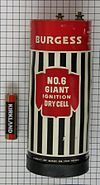
\includegraphics[height=.2\textheight]{R40-Burgess.jpg}\,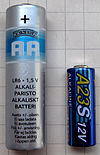
\includegraphics[height=.2\textheight]{100px-A23-AA-battery.jpg}}
\subtitle{The No. 6 and A23s of ``batteries included''}
\author{Kenneth Nielsen\inst{1}}
\institute
{
  \inst{1}%
  Center for Individual Nanoparticle Functionality (CINF)\\
  Institute of Physics\\
  Technical University of Denmark (DTU)
}
\date{
  Python and beers presentation,\\
  Aprils 29, 2015}
\subject{Computer Science}

\begin{document}

\frame{\titlepage}

\begin{frame}
  \frametitle{About me}
  \begin{itemize}
    \item My name is Kenneth Nielsen and I work at CINF
    \item Free and open source software (FOSS) enthusiast
    \item Use way too much time on python conference presentations on
      youtube
  \end{itemize}
  \begin{block}{Slides and examples}
    \center
    \footnotesize
    \texttt{git clone https://github.com/KennethNielsen/presentations.git}\newline
    \newline
    \texttt{https://github.com/KennethNielsen/presentations}
    \texttt{http://bit.ly/1FclzDR}
  \end{block}
\end{frame}

\begin{frame}
  \frametitle{Outline}

  A peak into some of the (maybe) lesser known gems of the standard library
  \begin{itemize}
  \item Convenient containers (... and more)
    \begin{itemize}
    \item defaultdict, Counter
    \end{itemize}
  \item Special operators for key functions (get rid of lambdas)
    \begin{itemize}
    \item itemgetter, attrgetter
    \end{itemize}
  \item Function tools
    \begin{itemize}
    \item partial
    \end{itemize}
  \item Part way between anonymous data and full classes
    \begin{itemize}
    \item namedtuple
    \end{itemize}
  \item Random stuff ;)
    \begin{itemize}
    \item choice
    \end{itemize}
  \end{itemize}
\end{frame}

\begin{frame}[fragile]
  \frametitle{defaultdict}
  \begin{minted}{python}
    from collections import defaultdict
    groups = defaultdict(default_callable)
  \end{minted}
  \begin{block}{\vspace*{-3ex}}
    A dictionary that will fill in values for unknown keys with
    defaults supplied by a callable
  \end{block}
  \begin{itemize}
  \item Useful e.g.\ for grouping, where you would otherwise have to
    write annoying first-item-init code
  \item Supply a callable when creating it, that will be called to ask
    for a default value
  \end{itemize}
  \begin{center}
    \texttt{LIVE! Example ex1\_default\_dict.py}
  \end{center}
\end{frame}

\begin{frame}[fragile]
  \frametitle{Counter}
  \begin{minted}{python}
    from collections import Counter
    counter = Counter()
  \end{minted}
  \begin{block}{\vspace*{-3ex}}
    A default dict with default value 0 (and some special counter
    relevant math)
  \end{block}
  \begin{itemize}
  \item Useful for counting!
  \item Can be added and subtracted
  \item Flattens out at 0 when subtracted
  \end{itemize}
  \begin{center}
    \texttt{LIVE! Example ex2\_counter.py}
  \end{center}
\end{frame}

\begin{frame}[fragile]
  \frametitle{itemgetter and attrgetter}
  \begin{minted}{python}
    from operator import itemgetter, attrgetter
  \end{minted}
  \begin{block}{\vspace*{-3ex}}
    Gives you a function that returns an element from an iterable or dict
    or a specific attribute from an object
  \end{block}
  \begin{itemize}
  \item {\color{darkred}EXTREMELY} usefull as \texttt{key} functions for
    \texttt{sort}, \texttt{sorted}, \texttt{min} and \texttt{max} ...
  \item ... especially because they make it possible to get rid of
    those pesky unreadable lambda expressions
  \end{itemize}
  \begin{center}
    \texttt{LIVE! Example ex3\_itemgetter\_attrgetter.py}
  \end{center}
\end{frame}

\begin{frame}[fragile]
  \frametitle{partial}
  \begin{minted}{python}
    from functools import partial
  \end{minted}
  \begin{block}{\vspace*{-3ex}}
    From original functions create new ones, where certain values in
    the original functions calls are already filled out
  \end{block}
  \begin{itemize}
  \item To call the same function a lot of times with one spcific
    argument
  \item To create custom functions that calls others with an argument
    filled out
  \end{itemize}
  \begin{center}
    \texttt{LIVE! Example ex4\_partial.py}\\
    \texttt{LIVE! Example ex5\_partial\_valve\_control.py}
  \end{center}
\end{frame}

\begin{frame}[fragile]
  \frametitle{namedtuple}
  \begin{minted}{python}
    from collections import namedtuple
  \end{minted}
  \begin{block}{\vspace*{-3ex}}
    Named tuples can be used to give your tuple like data structures a
    name and make it possible to access its values by names instead of
    index WITHOUT writing a class by hand for it
  \end{block}
  \begin{itemize}
  \item Usefull for naming data structures
  \item Usefull for getting . access instead of []
  \end{itemize}
  \begin{center}
    \texttt{LIVE! Example ex6\_namedtuple.py}
  \end{center}
\end{frame}

\begin{frame}[fragile]
  \frametitle{choise}
  \begin{minted}{python}
    from random import choice
  \end{minted}
  \begin{block}{\vspace*{-3ex}}
    Pick an element from an iterable at random.
  \end{block}
  \begin{center}
    \texttt{LIVE! Example ex7\_choice.py}
  \end{center}
\end{frame}

\begin{frame}
  \frametitle{Summary}
  \begin{itemize}
  \item The standard library has lots of little tools
  \item It is worth it to look for them, when needing them instead of
    rolling your own
  \end{itemize}
\end{frame}

% \begin{frame}[fragile]
%   \frametitle{Decorators}
% \begin{minted}{python}
% @my_decorator
% def my_function():
%     pass
% \end{minted}

\end{document}
